\renewcommand{\theequation}{\theenumi}
\begin{enumerate}[label=\thesubsection.\arabic*.,ref=\thesubsection.\theenumi]
\numberwithin{equation}{enumi}
	%
%
\item 
%
Draw a circle of radius 3 units.Take two points P and Q on one its extended diameter each at a distance of 7 units from its centre. Draw tangents to the circle from these two points P and Q. 
\\
\solution The given parameters are listed in Table \ref{tab:table1}
%
\begin{table}[!ht]
\begin{center}
\begin{tabular}{ | m{2cm} | m{2cm} |} 
\hline
 & Circle \\
\hline
Centre  & $\vec{O}$=\myvec{0\\0} \\ 
\hline
Radius & $r$=3  \\ 
\hline
Radius & $d$=7  \\ 
\hline
\end{tabular}
\end{center}
\caption{Input values}
\label{tab:table1}
\end{table}
%
\begin{lemma}
  \label{lemma/linman/circ/contact/final}
  The points of contact for the tangent drawn from a point 
%
\begin{align}
  \vec{P} = d\vec{e}_1, \text{ where } \vec{e}_1 = \myvec{1\\0}
  \end{align}
  %
  to the circle are given by 
  \begin{align}
    \vec{x} = \frac{r^2}{d}\vec{e}_1  \pm r\sqrt{1 - \frac{r^2}{d^2}} \vec{e}_2
    \label{linman/circ/contact/final}
   \end{align}
%   
\end{lemma}
If $\vec{x}$ be a point of contact for the tangent from $\vec{P}$, 
\begin{align}
PR &\perp RO
\\
 \implies (\vec{O}-\vec{x})^{\top} (\vec{x}-\vec{P}) &= 0
 \\
 \text{or, }  \vec{P}^{\top} \vec{x} &=\norm{\vec{x}}^2 = r^2
 \\
 \implies \vec{e}_1^{\top} \vec{x} &= \frac{r^2}{d}
  \end{align}
  $\because \vec{O} = 0$.  The above equation can be expressed in parametric form as 
 \begin{align}
  \vec{x} = \frac{r^2}{d}\vec{e}_1 + \lambda \vec{e}_2
  \label{linman/circ/contact}
 \end{align}
 Substituting the above in 
 \begin{align}
  \norm{\vec{x}}^2 = r^2,
 \end{align}
 yields
\begin{align}
\norm{\frac{r^2}{d}\vec{e}_1 + \lambda \vec{e}_2}^2&=r^2
\\
\implies \lambda^2 &= r^2\sbrak{1 - \frac{r^2}{d^2}}
\\
\text{or, }\lambda &= \pm r\sqrt{1 - \frac{r^2}{d^2}}
\end{align}
%
Substituting $\lambda $ in \eqref{linman/circ/contact} yields \eqref{linman/circ/contact/final}.  Fig.  \ref{fig:Tangent lines to circle of radius 3 units.} shows all possible tangents
and their points of contact after substituting the numerical values in \eqref{linman/circ/contact/final}.
%
\begin{figure}[ht]
  \centering
  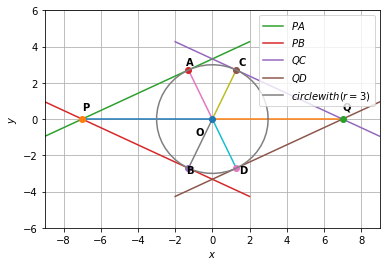
\includegraphics[width=\columnwidth]{solutions/su2021/circle/2/57/FIGURE3.png}
  \caption{Tangent lines to circle of radius 3 units.}
  \label{fig:Tangent lines to circle of radius 3 units.}
\end{figure}
%
\item Draw a  pair of tangents to a circle of radius 5 units  which are inclined to each other at an angle of $60\degree$.
\\
\solution  The angle between the tangents from $\vec{P}$ is given by 
\begin{lemma}
  Given a circle of radius $r$ and angle $\theta$ between the tangents, the intersection of the tangents and points of contact are
  given by Lemma   \ref{lemma/linman/circ/contact/final}  where 
  \begin{align}
    \implies d &= r\sin \frac{\theta}{2}
  \end{align}
%  
\end{lemma}
\begin{proof}
  From Fig.  \ref{fig:Tangent lines to circle of radius 3 units.},
\begin{align}
  \sin \frac{\theta}{2} &= \frac{r}{d}
  \\
  \implies d &= r\sin \frac{\theta}{2}
\end{align}
\end{proof}
Substituting numerical values and plotting, we obtain Fig. \ref{fig:Tangent lines to circle of radius 5 units.}.
%
\begin{figure}[ht]
  \centering
  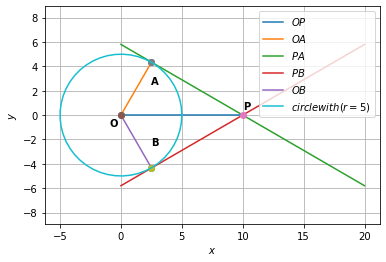
\includegraphics[width=\columnwidth]{solutions/su2021/circle/2/58/download.png}
  \caption{Tangent lines to circle of radius 5 units.}
  \label{fig:Tangent lines to circle of radius 5 units.}
\end{figure}   

\end{enumerate}
